% Options for packages loaded elsewhere
\PassOptionsToPackage{unicode}{hyperref}
\PassOptionsToPackage{hyphens}{url}
\PassOptionsToPackage{dvipsnames,svgnames,x11names}{xcolor}
%
\documentclass[
  letterpaper,
  DIV=11,
  numbers=noendperiod]{scrartcl}

\usepackage{amsmath,amssymb}
\usepackage{iftex}
\ifPDFTeX
  \usepackage[T1]{fontenc}
  \usepackage[utf8]{inputenc}
  \usepackage{textcomp} % provide euro and other symbols
\else % if luatex or xetex
  \usepackage{unicode-math}
  \defaultfontfeatures{Scale=MatchLowercase}
  \defaultfontfeatures[\rmfamily]{Ligatures=TeX,Scale=1}
\fi
\usepackage{lmodern}
\ifPDFTeX\else  
    % xetex/luatex font selection
\fi
% Use upquote if available, for straight quotes in verbatim environments
\IfFileExists{upquote.sty}{\usepackage{upquote}}{}
\IfFileExists{microtype.sty}{% use microtype if available
  \usepackage[]{microtype}
  \UseMicrotypeSet[protrusion]{basicmath} % disable protrusion for tt fonts
}{}
\makeatletter
\@ifundefined{KOMAClassName}{% if non-KOMA class
  \IfFileExists{parskip.sty}{%
    \usepackage{parskip}
  }{% else
    \setlength{\parindent}{0pt}
    \setlength{\parskip}{6pt plus 2pt minus 1pt}}
}{% if KOMA class
  \KOMAoptions{parskip=half}}
\makeatother
\usepackage{xcolor}
\setlength{\emergencystretch}{3em} % prevent overfull lines
\setcounter{secnumdepth}{-\maxdimen} % remove section numbering
% Make \paragraph and \subparagraph free-standing
\makeatletter
\ifx\paragraph\undefined\else
  \let\oldparagraph\paragraph
  \renewcommand{\paragraph}{
    \@ifstar
      \xxxParagraphStar
      \xxxParagraphNoStar
  }
  \newcommand{\xxxParagraphStar}[1]{\oldparagraph*{#1}\mbox{}}
  \newcommand{\xxxParagraphNoStar}[1]{\oldparagraph{#1}\mbox{}}
\fi
\ifx\subparagraph\undefined\else
  \let\oldsubparagraph\subparagraph
  \renewcommand{\subparagraph}{
    \@ifstar
      \xxxSubParagraphStar
      \xxxSubParagraphNoStar
  }
  \newcommand{\xxxSubParagraphStar}[1]{\oldsubparagraph*{#1}\mbox{}}
  \newcommand{\xxxSubParagraphNoStar}[1]{\oldsubparagraph{#1}\mbox{}}
\fi
\makeatother

\usepackage{color}
\usepackage{fancyvrb}
\newcommand{\VerbBar}{|}
\newcommand{\VERB}{\Verb[commandchars=\\\{\}]}
\DefineVerbatimEnvironment{Highlighting}{Verbatim}{commandchars=\\\{\}}
% Add ',fontsize=\small' for more characters per line
\usepackage{framed}
\definecolor{shadecolor}{RGB}{241,243,245}
\newenvironment{Shaded}{\begin{snugshade}}{\end{snugshade}}
\newcommand{\AlertTok}[1]{\textcolor[rgb]{0.68,0.00,0.00}{#1}}
\newcommand{\AnnotationTok}[1]{\textcolor[rgb]{0.37,0.37,0.37}{#1}}
\newcommand{\AttributeTok}[1]{\textcolor[rgb]{0.40,0.45,0.13}{#1}}
\newcommand{\BaseNTok}[1]{\textcolor[rgb]{0.68,0.00,0.00}{#1}}
\newcommand{\BuiltInTok}[1]{\textcolor[rgb]{0.00,0.23,0.31}{#1}}
\newcommand{\CharTok}[1]{\textcolor[rgb]{0.13,0.47,0.30}{#1}}
\newcommand{\CommentTok}[1]{\textcolor[rgb]{0.37,0.37,0.37}{#1}}
\newcommand{\CommentVarTok}[1]{\textcolor[rgb]{0.37,0.37,0.37}{\textit{#1}}}
\newcommand{\ConstantTok}[1]{\textcolor[rgb]{0.56,0.35,0.01}{#1}}
\newcommand{\ControlFlowTok}[1]{\textcolor[rgb]{0.00,0.23,0.31}{\textbf{#1}}}
\newcommand{\DataTypeTok}[1]{\textcolor[rgb]{0.68,0.00,0.00}{#1}}
\newcommand{\DecValTok}[1]{\textcolor[rgb]{0.68,0.00,0.00}{#1}}
\newcommand{\DocumentationTok}[1]{\textcolor[rgb]{0.37,0.37,0.37}{\textit{#1}}}
\newcommand{\ErrorTok}[1]{\textcolor[rgb]{0.68,0.00,0.00}{#1}}
\newcommand{\ExtensionTok}[1]{\textcolor[rgb]{0.00,0.23,0.31}{#1}}
\newcommand{\FloatTok}[1]{\textcolor[rgb]{0.68,0.00,0.00}{#1}}
\newcommand{\FunctionTok}[1]{\textcolor[rgb]{0.28,0.35,0.67}{#1}}
\newcommand{\ImportTok}[1]{\textcolor[rgb]{0.00,0.46,0.62}{#1}}
\newcommand{\InformationTok}[1]{\textcolor[rgb]{0.37,0.37,0.37}{#1}}
\newcommand{\KeywordTok}[1]{\textcolor[rgb]{0.00,0.23,0.31}{\textbf{#1}}}
\newcommand{\NormalTok}[1]{\textcolor[rgb]{0.00,0.23,0.31}{#1}}
\newcommand{\OperatorTok}[1]{\textcolor[rgb]{0.37,0.37,0.37}{#1}}
\newcommand{\OtherTok}[1]{\textcolor[rgb]{0.00,0.23,0.31}{#1}}
\newcommand{\PreprocessorTok}[1]{\textcolor[rgb]{0.68,0.00,0.00}{#1}}
\newcommand{\RegionMarkerTok}[1]{\textcolor[rgb]{0.00,0.23,0.31}{#1}}
\newcommand{\SpecialCharTok}[1]{\textcolor[rgb]{0.37,0.37,0.37}{#1}}
\newcommand{\SpecialStringTok}[1]{\textcolor[rgb]{0.13,0.47,0.30}{#1}}
\newcommand{\StringTok}[1]{\textcolor[rgb]{0.13,0.47,0.30}{#1}}
\newcommand{\VariableTok}[1]{\textcolor[rgb]{0.07,0.07,0.07}{#1}}
\newcommand{\VerbatimStringTok}[1]{\textcolor[rgb]{0.13,0.47,0.30}{#1}}
\newcommand{\WarningTok}[1]{\textcolor[rgb]{0.37,0.37,0.37}{\textit{#1}}}

\providecommand{\tightlist}{%
  \setlength{\itemsep}{0pt}\setlength{\parskip}{0pt}}\usepackage{longtable,booktabs,array}
\usepackage{calc} % for calculating minipage widths
% Correct order of tables after \paragraph or \subparagraph
\usepackage{etoolbox}
\makeatletter
\patchcmd\longtable{\par}{\if@noskipsec\mbox{}\fi\par}{}{}
\makeatother
% Allow footnotes in longtable head/foot
\IfFileExists{footnotehyper.sty}{\usepackage{footnotehyper}}{\usepackage{footnote}}
\makesavenoteenv{longtable}
\usepackage{graphicx}
\makeatletter
\def\maxwidth{\ifdim\Gin@nat@width>\linewidth\linewidth\else\Gin@nat@width\fi}
\def\maxheight{\ifdim\Gin@nat@height>\textheight\textheight\else\Gin@nat@height\fi}
\makeatother
% Scale images if necessary, so that they will not overflow the page
% margins by default, and it is still possible to overwrite the defaults
% using explicit options in \includegraphics[width, height, ...]{}
\setkeys{Gin}{width=\maxwidth,height=\maxheight,keepaspectratio}
% Set default figure placement to htbp
\makeatletter
\def\fps@figure{htbp}
\makeatother

\KOMAoption{captions}{tableheading}
\makeatletter
\@ifpackageloaded{tcolorbox}{}{\usepackage[skins,breakable]{tcolorbox}}
\@ifpackageloaded{fontawesome5}{}{\usepackage{fontawesome5}}
\definecolor{quarto-callout-color}{HTML}{909090}
\definecolor{quarto-callout-note-color}{HTML}{0758E5}
\definecolor{quarto-callout-important-color}{HTML}{CC1914}
\definecolor{quarto-callout-warning-color}{HTML}{EB9113}
\definecolor{quarto-callout-tip-color}{HTML}{00A047}
\definecolor{quarto-callout-caution-color}{HTML}{FC5300}
\definecolor{quarto-callout-color-frame}{HTML}{acacac}
\definecolor{quarto-callout-note-color-frame}{HTML}{4582ec}
\definecolor{quarto-callout-important-color-frame}{HTML}{d9534f}
\definecolor{quarto-callout-warning-color-frame}{HTML}{f0ad4e}
\definecolor{quarto-callout-tip-color-frame}{HTML}{02b875}
\definecolor{quarto-callout-caution-color-frame}{HTML}{fd7e14}
\makeatother
\makeatletter
\@ifpackageloaded{caption}{}{\usepackage{caption}}
\AtBeginDocument{%
\ifdefined\contentsname
  \renewcommand*\contentsname{Table of contents}
\else
  \newcommand\contentsname{Table of contents}
\fi
\ifdefined\listfigurename
  \renewcommand*\listfigurename{List of Figures}
\else
  \newcommand\listfigurename{List of Figures}
\fi
\ifdefined\listtablename
  \renewcommand*\listtablename{List of Tables}
\else
  \newcommand\listtablename{List of Tables}
\fi
\ifdefined\figurename
  \renewcommand*\figurename{Figure}
\else
  \newcommand\figurename{Figure}
\fi
\ifdefined\tablename
  \renewcommand*\tablename{Table}
\else
  \newcommand\tablename{Table}
\fi
}
\@ifpackageloaded{float}{}{\usepackage{float}}
\floatstyle{ruled}
\@ifundefined{c@chapter}{\newfloat{codelisting}{h}{lop}}{\newfloat{codelisting}{h}{lop}[chapter]}
\floatname{codelisting}{Listing}
\newcommand*\listoflistings{\listof{codelisting}{List of Listings}}
\makeatother
\makeatletter
\makeatother
\makeatletter
\@ifpackageloaded{caption}{}{\usepackage{caption}}
\@ifpackageloaded{subcaption}{}{\usepackage{subcaption}}
\makeatother

\ifLuaTeX
  \usepackage{selnolig}  % disable illegal ligatures
\fi
\usepackage{bookmark}

\IfFileExists{xurl.sty}{\usepackage{xurl}}{} % add URL line breaks if available
\urlstyle{same} % disable monospaced font for URLs
\hypersetup{
  pdftitle={Data Visualisation Tutorial},
  pdfauthor={Dr Kanthu Joseph Mhango},
  colorlinks=true,
  linkcolor={blue},
  filecolor={Maroon},
  citecolor={Blue},
  urlcolor={Blue},
  pdfcreator={LaTeX via pandoc}}


\title{Data Visualisation Tutorial}
\usepackage{etoolbox}
\makeatletter
\providecommand{\subtitle}[1]{% add subtitle to \maketitle
  \apptocmd{\@title}{\par {\large #1 \par}}{}{}
}
\makeatother
\subtitle{A self-guided Quarto tutorial}
\author{Dr Kanthu Joseph Mhango}
\date{2026-01-23}

\begin{document}
\maketitle


\subsection{Welcome (read this first)}\label{welcome-read-this-first}

This tutorial assumes \textbf{you are at the beginning of your journey
with R} and \textbf{you are seeing ggplot2 for the first time}. That is
completely fine. We will be very slow, very explicit, and we will repeat
the same ideas until they feel familiar.

\subsubsection{What ``Base R plotting'' means (the default plotting
engine)}\label{what-base-r-plotting-means-the-default-plotting-engine}

R comes with a built-in plotting system. It is often called \textbf{Base
R graphics}.

\begin{itemize}
\tightlist
\item
  It is the \textbf{default} because it is included with R.
\item
  You do \textbf{not} need to install anything to use it.
\item
  You usually build a plot by giving R \textbf{step-by-step drawing
  instructions}:

  \begin{itemize}
  \tightlist
  \item
    ``draw the points''
  \item
    ``now draw a line''
  \item
    ``now add a legend''
  \item
    ``now change the axis labels''
  \end{itemize}
\end{itemize}

This is called an \textbf{imperative} style: you tell the computer what
to do next, like giving directions.

\subsubsection{What ggplot2 is (and why people use
it)}\label{what-ggplot2-is-and-why-people-use-it}

\texttt{ggplot2} is a very popular R package for plots. It is based on
an idea called the \textbf{Grammar of Graphics}.

The beginner-friendly meaning is:

\begin{itemize}
\tightlist
\item
  A plot is not just a picture.
\item
  A plot is a \textbf{structured description} of how data becomes marks
  (points/lines/bars) on axes.
\end{itemize}

So instead of manually drawing each element, you \emph{describe the
meaning}:

\begin{itemize}
\tightlist
\item
  which dataset
\item
  which variable goes on x and y
\item
  which variable controls colour (or size, or shape)
\item
  what mark to draw (points? lines? bars?)
\item
  whether to split into panels (facets)
\end{itemize}

This is called a \textbf{declarative} style: you declare what the plot
means, and ggplot draws it.

\subsubsection{The big advantage of ggplot2
(consistency)}\label{the-big-advantage-of-ggplot2-consistency}

Base R can make good plots, but complex plots often require many manual
steps.

ggplot2 is easier for many people because the code is
\textbf{consistent}:

\begin{itemize}
\tightlist
\item
  the beginning is almost always \texttt{ggplot(data,\ aes(...))}
\item
  each new visual layer looks like \texttt{+\ geom\_*()}
\item
  legends usually appear automatically from the mapping in
  \texttt{aes()}
\item
  multi-panel plots are usually one line: \texttt{facet\_*()}
\end{itemize}

\subsubsection{The anatomy of ggplot code (learn this
pattern)}\label{the-anatomy-of-ggplot-code-learn-this-pattern}

Most ggplot graphs follow this repeatable ``sentence'':

\begin{Shaded}
\begin{Highlighting}[]
\FunctionTok{ggplot}\NormalTok{(DATA, }\FunctionTok{aes}\NormalTok{(MAPPINGS)) }\SpecialCharTok{+}
  \FunctionTok{geom\_SOMETHING}\NormalTok{(...) }\SpecialCharTok{+}
  \FunctionTok{scale\_SOMETHING}\NormalTok{(...) }\SpecialCharTok{+}
  \FunctionTok{coord\_SOMETHING}\NormalTok{(...) }\SpecialCharTok{+}
  \FunctionTok{facet\_SOMETHING}\NormalTok{(...) }\SpecialCharTok{+}
  \FunctionTok{labs}\NormalTok{(...) }\SpecialCharTok{+}
  \FunctionTok{theme\_SOMETHING}\NormalTok{(...)}
\end{Highlighting}
\end{Shaded}

Now in plain English:

\begin{itemize}
\tightlist
\item
  \texttt{ggplot(DATA,\ ...)}: ``I am making a plot from this dataset.''
\item
  \texttt{aes(...)}: ``Here is what variables mean visually (x, y,
  colour, etc.).''
\item
  \texttt{geom\_*()}: ``Here is how to draw the data (points, lines,
  bars\ldots).''
\item
  \texttt{scale\_*()}: ``Here is how to translate values into
  colours/axes/labels.''
\item
  \texttt{coord\_*()}: ``Here is the coordinate system / viewing
  window.''
\item
  \texttt{facet\_*()}: ``Split into multiple panels (small multiples).''
\item
  \texttt{labs(...)}: ``Titles and axis labels so humans can read it.''
\item
  \texttt{theme\_*()}: ``Styling rules (font sizes, background, grid
  lines).''
\end{itemize}

\subsubsection{How this tutorial works (Base R → think → ggplot →
discuss)}\label{how-this-tutorial-works-base-r-think-ggplot-discuss}

Every module follows the same rhythm:

\begin{enumerate}
\def\labelenumi{\arabic{enumi}.}
\tightlist
\item
  \textbf{We show the Base R version first} (manual drawing, step by
  step).
\item
  \textbf{You pause and predict the ggplot version} (you try to guess
  the pieces).
\item
  \textbf{We show the ggplot version} (using the same grammar pattern).
\item
  \textbf{We discuss} the differences in very simple language.
\end{enumerate}

\subsection{Setup}\label{setup}

\subsubsection{Load packages and set
defaults}\label{load-packages-and-set-defaults}

\begin{Shaded}
\begin{Highlighting}[]
\FunctionTok{library}\NormalTok{(ggplot2)}

\FunctionTok{set.seed}\NormalTok{(}\DecValTok{123}\NormalTok{)}

\CommentTok{\# this below code is optional, it just makes plots consistent in this tutorial}
\NormalTok{knitr}\SpecialCharTok{::}\NormalTok{opts\_chunk}\SpecialCharTok{$}\FunctionTok{set}\NormalTok{(}
  \AttributeTok{fig.width =} \DecValTok{8}\NormalTok{,}
  \AttributeTok{fig.height =} \FloatTok{4.8}\NormalTok{,}
  \AttributeTok{fig.align =} \StringTok{"center"}
\NormalTok{)}
\end{Highlighting}
\end{Shaded}

\subsubsection{What we will use}\label{what-we-will-use}

\begin{itemize}
\tightlist
\item
  Dataset: \texttt{iris}
\item
  Tools: \textbf{Base R} graphics and \textbf{ggplot2}
\end{itemize}

\begin{Shaded}
\begin{Highlighting}[]
\FunctionTok{head}\NormalTok{(iris)}
\end{Highlighting}
\end{Shaded}

\begin{verbatim}
  Sepal.Length Sepal.Width Petal.Length Petal.Width Species
1          5.1         3.5          1.4         0.2  setosa
2          4.9         3.0          1.4         0.2  setosa
3          4.7         3.2          1.3         0.2  setosa
4          4.6         3.1          1.5         0.2  setosa
5          5.0         3.6          1.4         0.2  setosa
6          5.4         3.9          1.7         0.4  setosa
\end{verbatim}

\begin{tcolorbox}[enhanced jigsaw, opacitybacktitle=0.6, left=2mm, bottomrule=.15mm, coltitle=black, opacityback=0, toptitle=1mm, title=\textcolor{quarto-callout-note-color}{\faInfo}\hspace{0.5em}{Note}, colbacktitle=quarto-callout-note-color!10!white, breakable, colback=white, rightrule=.15mm, colframe=quarto-callout-note-color-frame, bottomtitle=1mm, arc=.35mm, titlerule=0mm, toprule=.15mm, leftrule=.75mm]

\textbf{A beginner-friendly way to think about good visualisation}

Every plot should answer a question. In this tutorial, we repeatedly
ask:

\begin{itemize}
\tightlist
\item
  What comparison or pattern should the reader see \emph{in one glance}?
\item
  What is the \textbf{main visual signal} (x position, y position,
  colour, panels, text)?
\item
  What is the \textbf{most likely misread} (and how do we prevent it)?
\end{itemize}

\end{tcolorbox}

\begin{center}\rule{0.5\linewidth}{0.5pt}\end{center}

\subsection{1 --- Scatter plot with legend + reference
line}\label{scatter-plot-with-legend-reference-line}

\subsubsection{Goal}\label{goal}

Create a scatter plot of:

\begin{itemize}
\tightlist
\item
  x = \texttt{Sepal.Length}
\item
  y = \texttt{Petal.Length}
\item
  colour by \texttt{Species}
\end{itemize}

Add:

\begin{itemize}
\tightlist
\item
  a \textbf{dashed 1:1 reference line}
\item
  a \textbf{legend} with clear labels
\item
  axis labels with \textbf{units}
\end{itemize}

\subsubsection{Step 1: Base R version (shown
first)}\label{step-1-base-r-version-shown-first}

In Base R, you build a plot by telling R what to draw \textbf{one step
at a time}.

Read the next code like a recipe:

\begin{itemize}
\tightlist
\item
  \texttt{plot(...)} draws the points
\item
  \texttt{abline(...)} draws the dashed 1:1 line
\item
  \texttt{legend(...)} creates the legend
\end{itemize}

Here is the Base R code:

\begin{Shaded}
\begin{Highlighting}[]
\FunctionTok{plot}\NormalTok{(}
\NormalTok{  iris}\SpecialCharTok{$}\NormalTok{Sepal.Length, iris}\SpecialCharTok{$}\NormalTok{Petal.Length,}
  \AttributeTok{col =} \FunctionTok{as.numeric}\NormalTok{(iris}\SpecialCharTok{$}\NormalTok{Species),}
  \AttributeTok{pch =} \DecValTok{16}\NormalTok{,}
  \AttributeTok{xlab =} \StringTok{"Sepal Length (cm)"}\NormalTok{,}
  \AttributeTok{ylab =} \StringTok{"Petal Length (cm)"}\NormalTok{,}
  \AttributeTok{main =} \StringTok{"Scatter with Dashed Reference Line"}
\NormalTok{)}

\FunctionTok{abline}\NormalTok{(}\AttributeTok{a =} \DecValTok{0}\NormalTok{, }\AttributeTok{b =} \DecValTok{1}\NormalTok{, }\AttributeTok{lty =} \DecValTok{2}\NormalTok{)}

\FunctionTok{legend}\NormalTok{(}
  \StringTok{"topleft"}\NormalTok{,}
  \AttributeTok{legend =} \FunctionTok{levels}\NormalTok{(iris}\SpecialCharTok{$}\NormalTok{Species),}
  \AttributeTok{col =} \DecValTok{1}\SpecialCharTok{:}\DecValTok{3}\NormalTok{,}
  \AttributeTok{pch =} \DecValTok{16}\NormalTok{,}
  \AttributeTok{title =} \StringTok{"Species"}
\NormalTok{)}
\end{Highlighting}
\end{Shaded}

\begin{center}
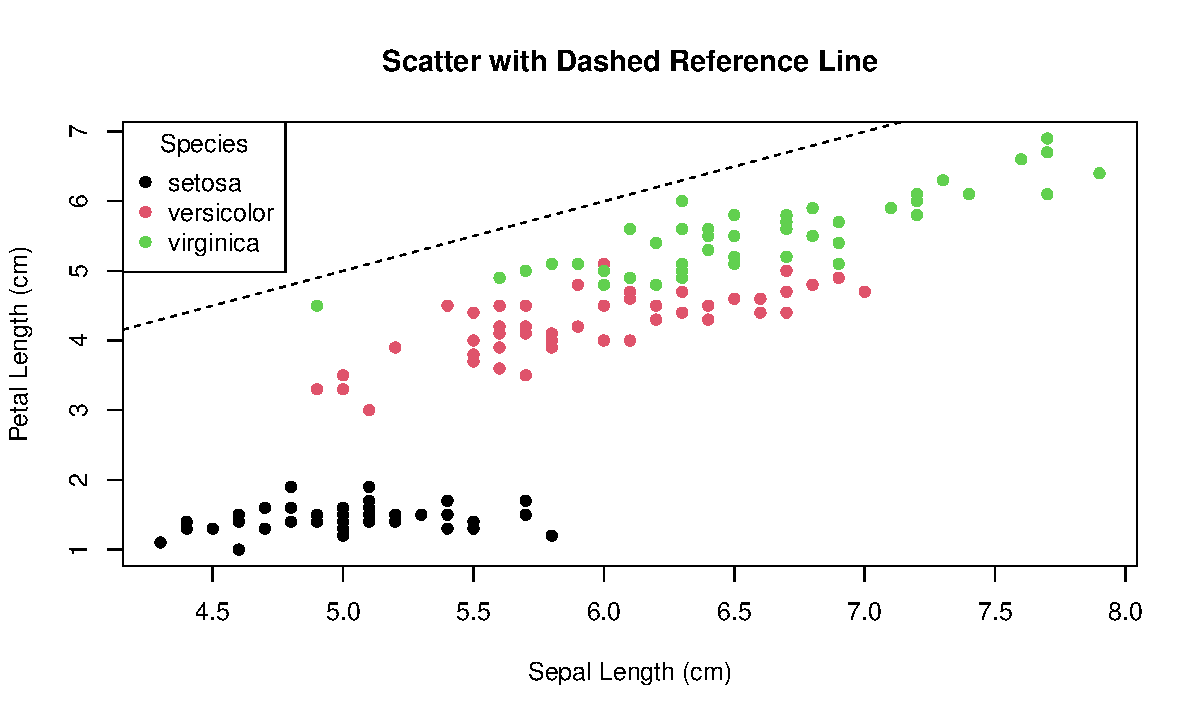
\includegraphics{vistut_files/figure-pdf/unnamed-chunk-3-1.pdf}
\end{center}

\begin{tcolorbox}[enhanced jigsaw, opacitybacktitle=0.6, left=2mm, bottomrule=.15mm, coltitle=black, opacityback=0, toptitle=1mm, title=\textcolor{quarto-callout-note-color}{\faInfo}\hspace{0.5em}{Note}, colbacktitle=quarto-callout-note-color!10!white, breakable, colback=white, rightrule=.15mm, colframe=quarto-callout-note-color-frame, bottomtitle=1mm, arc=.35mm, titlerule=0mm, toprule=.15mm, leftrule=.75mm]

\textbf{Principles used}

\begin{itemize}
\tightlist
\item
  \textbf{Reference lines are arguments}: a 1:1 line creates an
  immediate benchmark for ``above vs below''.
\item
  \textbf{Figure--ground}: keep non-data ink light (dashed line) so
  points remain the focus.
\item
  \textbf{Legends must be decodable}: if colour encodes groups, the
  legend must be present and readable.
\end{itemize}

\end{tcolorbox}

\subsubsection{Step 2: pause and predict the ggplot2
version}\label{step-2-pause-and-predict-the-ggplot2-version}

Now we do the same figure in ggplot2. Before looking at the solution,
pause and ask:

\begin{itemize}
\tightlist
\item
  What is the dataset? (\textbf{iris})
\item
  What goes on x? (\textbf{Sepal.Length})
\item
  What goes on y? (\textbf{Petal.Length})
\item
  What does colour mean? (\textbf{Species})
\item
  What do we draw? (\textbf{points})
\item
  What extra guide line do we add? (\textbf{a 1:1 line})
\end{itemize}

Try writing a ggplot ``sentence'' in your head first. If you want to
sketch code, use this practice chunk (it will not run):

\begin{Shaded}
\begin{Highlighting}[]
\CommentTok{\# ggplot(iris, aes(x = Sepal.Length, y = Petal.Length, colour = Species)) +}
\CommentTok{\#   geom\_point(...) +}
\CommentTok{\#   geom\_abline(...) +}
\CommentTok{\#   labs(...) +}
\CommentTok{\#   theme\_...()}
\end{Highlighting}
\end{Shaded}

\subsubsection{Step 3: ggplot2 version
(solution)}\label{step-3-ggplot2-version-solution}

\begin{Shaded}
\begin{Highlighting}[]
\FunctionTok{ggplot}\NormalTok{(iris, }\FunctionTok{aes}\NormalTok{(Sepal.Length, Petal.Length, }\AttributeTok{colour =}\NormalTok{ Species)) }\SpecialCharTok{+}
  \FunctionTok{geom\_point}\NormalTok{(}\AttributeTok{size =} \DecValTok{2}\NormalTok{, }\AttributeTok{alpha =} \FloatTok{0.85}\NormalTok{) }\SpecialCharTok{+}
  \FunctionTok{geom\_abline}\NormalTok{(}\AttributeTok{intercept =} \DecValTok{0}\NormalTok{, }\AttributeTok{slope =} \DecValTok{1}\NormalTok{, }\AttributeTok{linetype =} \DecValTok{2}\NormalTok{) }\SpecialCharTok{+}
  \FunctionTok{labs}\NormalTok{(}
    \AttributeTok{x =} \StringTok{"Sepal Length (cm)"}\NormalTok{,}
    \AttributeTok{y =} \StringTok{"Petal Length (cm)"}\NormalTok{,}
    \AttributeTok{colour =} \StringTok{"Species"}\NormalTok{,}
    \AttributeTok{title =} \StringTok{"Scatter with Dashed Reference Line"}
\NormalTok{  ) }\SpecialCharTok{+}
  \FunctionTok{theme\_minimal}\NormalTok{(}\AttributeTok{base\_size =} \DecValTok{13}\NormalTok{)}
\end{Highlighting}
\end{Shaded}

\begin{center}
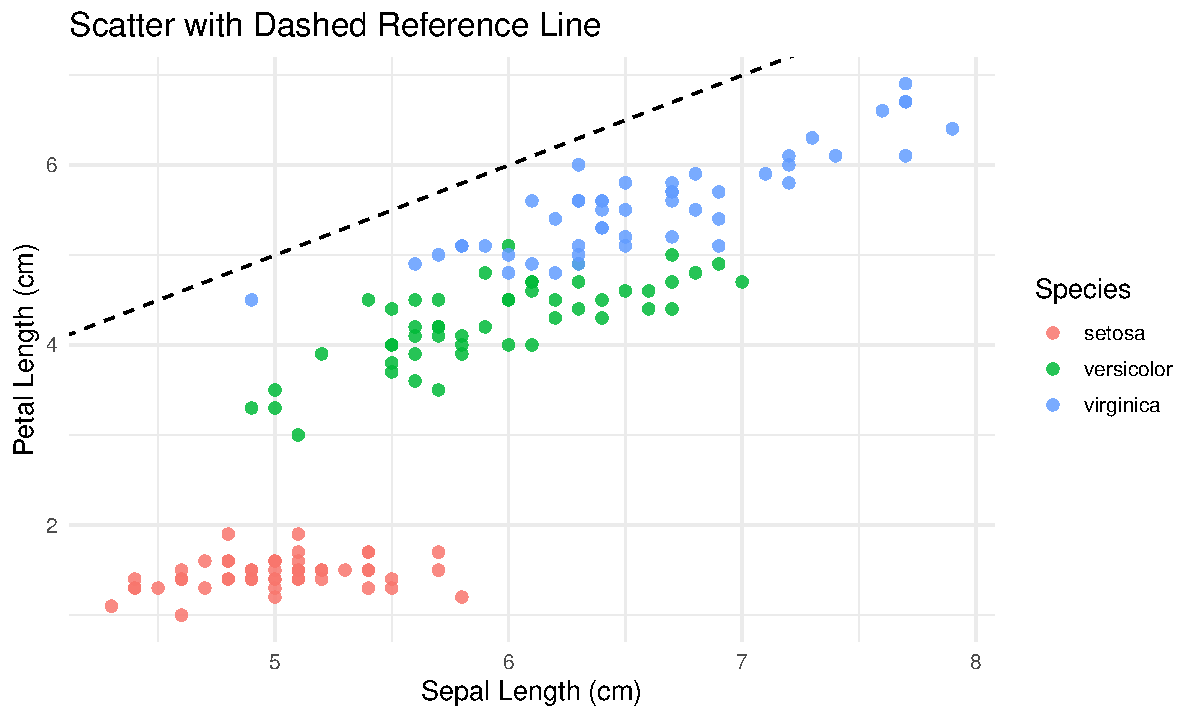
\includegraphics{vistut_files/figure-pdf/unnamed-chunk-5-1.pdf}
\end{center}

\subsubsection{Step 4: discussion (what you should
notice)}\label{step-4-discussion-what-you-should-notice}

\begin{itemize}
\tightlist
\item
  In \textbf{Base R}, you built the plot by issuing separate commands.
\item
  In \textbf{ggplot2}, you declared the meaning once (inside
  \texttt{aes(...)}), and ggplot handled the legend automatically.
\item
  The ggplot version is easier to extend consistently: if you want
  another layer later, you add another line starting with \texttt{+}.
\end{itemize}

\begin{center}\rule{0.5\linewidth}{0.5pt}\end{center}

\subsection{2 --- Grouped line plot}\label{grouped-line-plot}

\subsubsection{Goal}\label{goal-1}

Plot three lines (one per species) over an index \texttt{x\ =\ 1:5}
using the provided means:

\begin{Shaded}
\begin{Highlighting}[]
\NormalTok{x }\OtherTok{\textless{}{-}} \DecValTok{1}\SpecialCharTok{:}\DecValTok{5}
\NormalTok{setosa\_means     }\OtherTok{\textless{}{-}} \FunctionTok{c}\NormalTok{(}\FloatTok{1.4}\NormalTok{, }\FloatTok{1.45}\NormalTok{, }\FloatTok{1.5}\NormalTok{, }\FloatTok{1.55}\NormalTok{, }\FloatTok{1.6}\NormalTok{)}
\NormalTok{versicolor\_means }\OtherTok{\textless{}{-}} \FunctionTok{c}\NormalTok{(}\FloatTok{4.0}\NormalTok{, }\FloatTok{4.1}\NormalTok{, }\FloatTok{4.2}\NormalTok{, }\FloatTok{4.3}\NormalTok{, }\FloatTok{4.4}\NormalTok{)}
\NormalTok{virginica\_means  }\OtherTok{\textless{}{-}} \FunctionTok{c}\NormalTok{(}\FloatTok{5.5}\NormalTok{, }\FloatTok{5.6}\NormalTok{, }\FloatTok{5.7}\NormalTok{, }\FloatTok{5.8}\NormalTok{, }\FloatTok{5.9}\NormalTok{)}
\end{Highlighting}
\end{Shaded}

\subsubsection{Step 1: Base R version (shown
first)}\label{step-1-base-r-version-shown-first-1}

In Base R, a ``grouped line plot'' often means:

\begin{itemize}
\tightlist
\item
  plot the first line with \texttt{plot(...,\ type\ =\ "l")}
\item
  then manually add other lines with \texttt{lines(...)}
\item
  then manually add a legend
\end{itemize}

Here is the Base R code:

\begin{Shaded}
\begin{Highlighting}[]
\FunctionTok{plot}\NormalTok{(}
\NormalTok{  x, setosa\_means,}
  \AttributeTok{type =} \StringTok{"l"}\NormalTok{, }\AttributeTok{lwd =} \DecValTok{2}\NormalTok{, }\AttributeTok{col =} \DecValTok{1}\NormalTok{,}
  \AttributeTok{ylim =} \FunctionTok{c}\NormalTok{(}\DecValTok{1}\NormalTok{, }\DecValTok{6}\NormalTok{),}
  \AttributeTok{xlab =} \StringTok{"Index"}\NormalTok{, }\AttributeTok{ylab =} \StringTok{"Mean Petal Length"}\NormalTok{,}
  \AttributeTok{main =} \StringTok{"Grouped Line Plot by Species"}
\NormalTok{)}
\FunctionTok{lines}\NormalTok{(x, versicolor\_means, }\AttributeTok{col =} \DecValTok{2}\NormalTok{, }\AttributeTok{lwd =} \DecValTok{2}\NormalTok{)}
\FunctionTok{lines}\NormalTok{(x, virginica\_means,  }\AttributeTok{col =} \DecValTok{3}\NormalTok{, }\AttributeTok{lwd =} \DecValTok{2}\NormalTok{)}
\FunctionTok{legend}\NormalTok{(}
  \StringTok{"topleft"}\NormalTok{,}
  \AttributeTok{legend =} \FunctionTok{c}\NormalTok{(}\StringTok{"setosa"}\NormalTok{, }\StringTok{"versicolor"}\NormalTok{, }\StringTok{"virginica"}\NormalTok{),}
  \AttributeTok{col =} \DecValTok{1}\SpecialCharTok{:}\DecValTok{3}\NormalTok{, }\AttributeTok{lwd =} \DecValTok{2}\NormalTok{, }\AttributeTok{title =} \StringTok{"Species"}
\NormalTok{)}
\end{Highlighting}
\end{Shaded}

\begin{center}
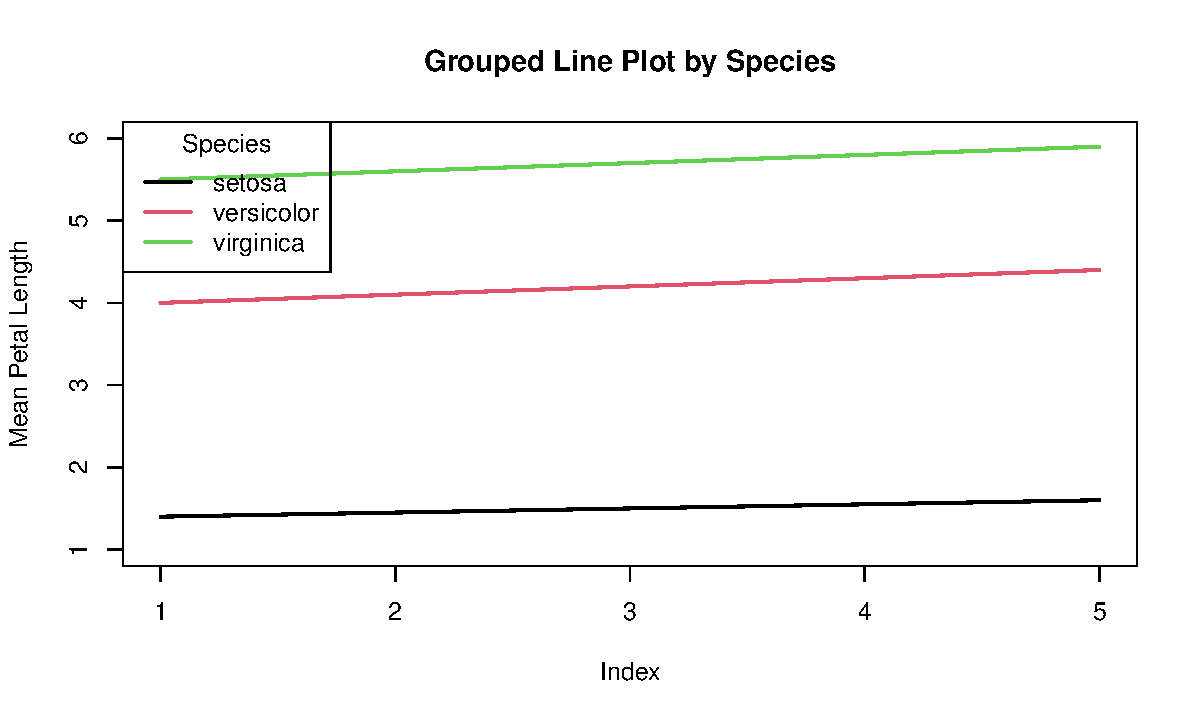
\includegraphics{vistut_files/figure-pdf/unnamed-chunk-7-1.pdf}
\end{center}

\subsubsection{Step 2: pause and predict the ggplot2
version}\label{step-2-pause-and-predict-the-ggplot2-version-1}

Now think in ggplot terms.

In ggplot2, you strongly prefer your data to be in a simple table where:

\begin{itemize}
\tightlist
\item
  each row is one observation you want to draw
\item
  each column is a variable (x, y, group, etc.)
\end{itemize}

So, to draw three lines, we should build a table with:

\begin{itemize}
\tightlist
\item
  \texttt{Index} (x)
\item
  \texttt{MeanPetalLength} (y)
\item
  \texttt{Species} (which line / which colour)
\end{itemize}

\subsubsection{Step 3: ggplot2 version
(solution)}\label{step-3-ggplot2-version-solution-1}

First we create a tidy dataframe:

\begin{Shaded}
\begin{Highlighting}[]
\NormalTok{means\_df }\OtherTok{\textless{}{-}} \FunctionTok{data.frame}\NormalTok{(}
  \AttributeTok{Index =} \FunctionTok{rep}\NormalTok{(x, }\AttributeTok{times =} \DecValTok{3}\NormalTok{),}
  \AttributeTok{Species =} \FunctionTok{rep}\NormalTok{(}\FunctionTok{c}\NormalTok{(}\StringTok{"setosa"}\NormalTok{, }\StringTok{"versicolor"}\NormalTok{, }\StringTok{"virginica"}\NormalTok{), }\AttributeTok{each =} \FunctionTok{length}\NormalTok{(x)),}
  \AttributeTok{MeanPetalLength =} \FunctionTok{c}\NormalTok{(setosa\_means, versicolor\_means, virginica\_means)}
\NormalTok{)}

\FunctionTok{head}\NormalTok{(means\_df)}
\end{Highlighting}
\end{Shaded}

\begin{verbatim}
  Index    Species MeanPetalLength
1     1     setosa            1.40
2     2     setosa            1.45
3     3     setosa            1.50
4     4     setosa            1.55
5     5     setosa            1.60
6     1 versicolor            4.00
\end{verbatim}

Now we plot it with the repeatable ggplot pattern:

\begin{Shaded}
\begin{Highlighting}[]
\FunctionTok{ggplot}\NormalTok{(means\_df, }\FunctionTok{aes}\NormalTok{(}\AttributeTok{x =}\NormalTok{ Index, }\AttributeTok{y =}\NormalTok{ MeanPetalLength, }\AttributeTok{colour =}\NormalTok{ Species)) }\SpecialCharTok{+}
  \FunctionTok{geom\_line}\NormalTok{(}\AttributeTok{linewidth =} \FloatTok{1.2}\NormalTok{) }\SpecialCharTok{+}
  \FunctionTok{geom\_point}\NormalTok{(}\AttributeTok{size =} \DecValTok{2}\NormalTok{) }\SpecialCharTok{+}
  \FunctionTok{labs}\NormalTok{(}
    \AttributeTok{x =} \StringTok{"Index"}\NormalTok{,}
    \AttributeTok{y =} \StringTok{"Mean Petal Length"}\NormalTok{,}
    \AttributeTok{colour =} \StringTok{"Species"}\NormalTok{,}
    \AttributeTok{title =} \StringTok{"Grouped Line Plot by Species (ggplot2)"}
\NormalTok{  ) }\SpecialCharTok{+}
  \FunctionTok{theme\_minimal}\NormalTok{(}\AttributeTok{base\_size =} \DecValTok{13}\NormalTok{)}
\end{Highlighting}
\end{Shaded}

\begin{center}
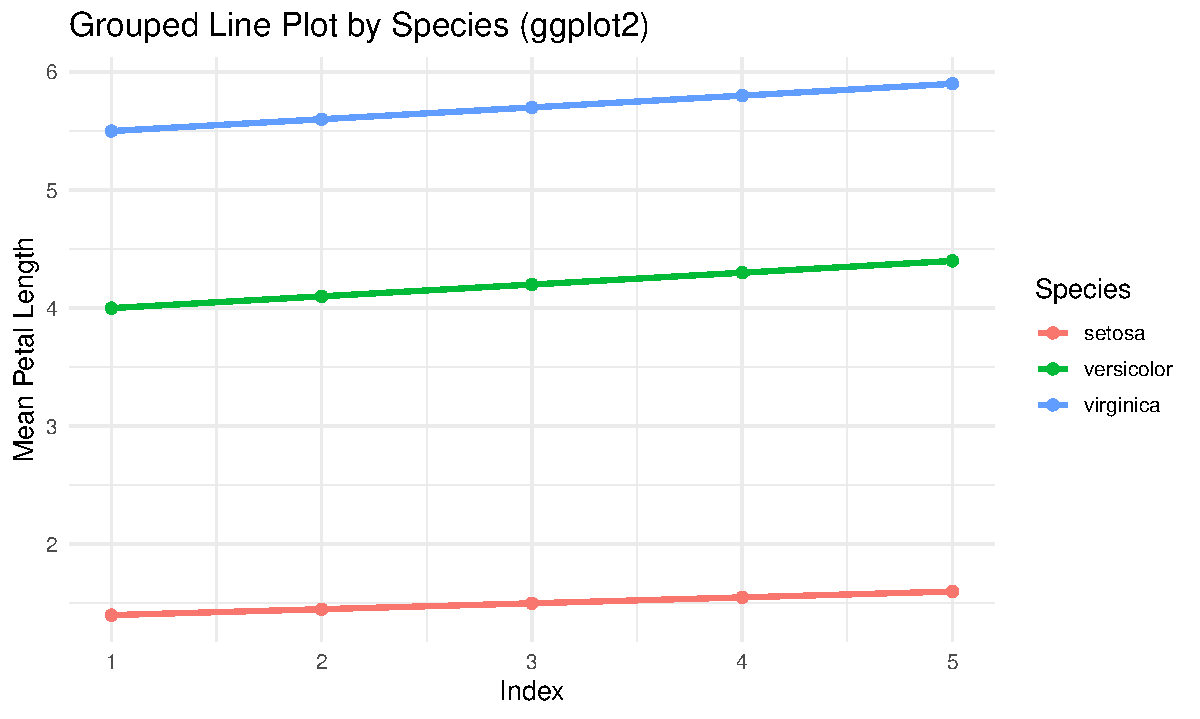
\includegraphics{vistut_files/figure-pdf/unnamed-chunk-9-1.pdf}
\end{center}

\subsubsection{Step 4: discussion (why ggplot feels easier
here)}\label{step-4-discussion-why-ggplot-feels-easier-here}

\begin{itemize}
\tightlist
\item
  In \textbf{Base R}, you wrote separate code for each group
  (\texttt{setosa}, \texttt{versicolor}, \texttt{virginica}).
\item
  In \textbf{ggplot2}, groups are just \textbf{values in a column}
  (\texttt{Species}), so adding a new group would just mean adding rows
  to the data.
\item
  The legend is automatic again because we mapped
  \texttt{colour\ =\ Species}.
\end{itemize}

\begin{tcolorbox}[enhanced jigsaw, opacitybacktitle=0.6, left=2mm, bottomrule=.15mm, coltitle=black, opacityback=0, toptitle=1mm, title=\textcolor{quarto-callout-note-color}{\faInfo}\hspace{0.5em}{Note}, colbacktitle=quarto-callout-note-color!10!white, breakable, colback=white, rightrule=.15mm, colframe=quarto-callout-note-color-frame, bottomtitle=1mm, arc=.35mm, titlerule=0mm, toprule=.15mm, leftrule=.75mm]

\textbf{Principles used}

\begin{itemize}
\tightlist
\item
  \textbf{Proximity + continuity}: line plots are best when the story is
  ``change across ordered x''.
\item
  \textbf{Common scales}: fixed \texttt{ylim} (Base R) prevents
  misleading comparisons caused by autoscaling.
\end{itemize}

\end{tcolorbox}

\begin{center}\rule{0.5\linewidth}{0.5pt}\end{center}

\subsection{3 --- Labelled plot (text
marks)}\label{labelled-plot-text-marks}

\subsubsection{Goal}\label{goal-2}

Replace points with initials:

\begin{itemize}
\tightlist
\item
  setosa → ``s''
\item
  versicolor → ``v''
\item
  virginica → ``v'' (problem!)
\end{itemize}

This exposes a design issue: \textbf{labels can collide} and
\textbf{symbols can be ambiguous}.

\subsubsection{Step 1: Base R version (shown
first)}\label{step-1-base-r-version-shown-first-2}

In Base R, a labelled plot usually works like this:

\begin{itemize}
\tightlist
\item
  first you create a blank plotting area (\texttt{type\ =\ "n"})
\item
  then you place text labels using \texttt{text(...)}
\end{itemize}

Here we label each point using the first letter of the species name.

\begin{tcolorbox}[enhanced jigsaw, opacitybacktitle=0.6, left=2mm, bottomrule=.15mm, coltitle=black, opacityback=0, toptitle=1mm, title=\textcolor{quarto-callout-tip-color}{\faLightbulb}\hspace{0.5em}{Solution (Base R)}, colbacktitle=quarto-callout-tip-color!10!white, breakable, colback=white, rightrule=.15mm, colframe=quarto-callout-tip-color-frame, bottomtitle=1mm, arc=.35mm, titlerule=0mm, toprule=.15mm, leftrule=.75mm]

\begin{Shaded}
\begin{Highlighting}[]
\FunctionTok{plot}\NormalTok{(}
\NormalTok{  iris}\SpecialCharTok{$}\NormalTok{Sepal.Length, iris}\SpecialCharTok{$}\NormalTok{Petal.Length,}
  \AttributeTok{type =} \StringTok{"n"}\NormalTok{,}
  \AttributeTok{xlab =} \StringTok{"Sepal Length"}\NormalTok{,}
  \AttributeTok{ylab =} \StringTok{"Petal Length"}\NormalTok{,}
  \AttributeTok{main =} \StringTok{"Labelled Plot (Initials Instead of Points)"}
\NormalTok{)}

\FunctionTok{text}\NormalTok{(}
\NormalTok{  iris}\SpecialCharTok{$}\NormalTok{Sepal.Length, iris}\SpecialCharTok{$}\NormalTok{Petal.Length,}
  \AttributeTok{labels =} \FunctionTok{substr}\NormalTok{(iris}\SpecialCharTok{$}\NormalTok{Species, }\DecValTok{1}\NormalTok{, }\DecValTok{1}\NormalTok{),}
  \AttributeTok{col =} \FunctionTok{as.numeric}\NormalTok{(iris}\SpecialCharTok{$}\NormalTok{Species)}
\NormalTok{)}

\FunctionTok{legend}\NormalTok{(}
  \StringTok{"topleft"}\NormalTok{,}
  \AttributeTok{legend =} \FunctionTok{levels}\NormalTok{(iris}\SpecialCharTok{$}\NormalTok{Species),}
  \AttributeTok{col =} \DecValTok{1}\SpecialCharTok{:}\DecValTok{3}\NormalTok{, }\AttributeTok{pch =} \DecValTok{15}\NormalTok{, }\AttributeTok{title =} \StringTok{"Species"}
\NormalTok{)}
\end{Highlighting}
\end{Shaded}

\begin{center}
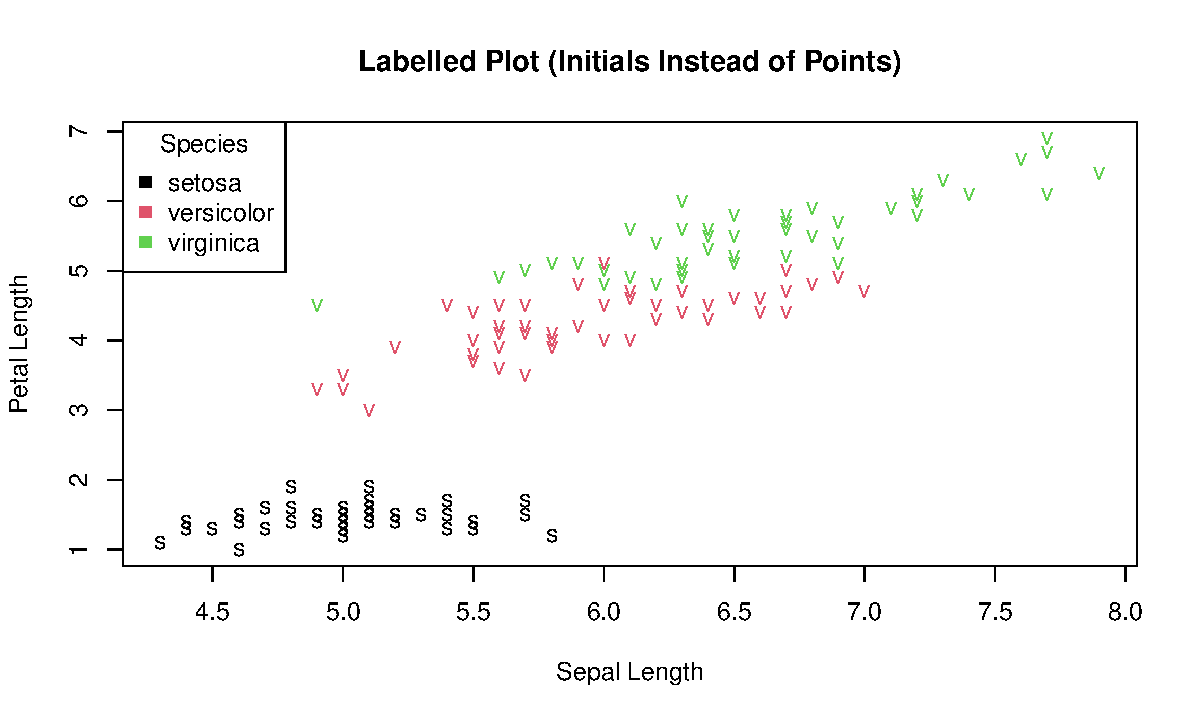
\includegraphics{vistut_files/figure-pdf/unnamed-chunk-10-1.pdf}
\end{center}

\end{tcolorbox}

\subsubsection{Step 2: pause and predict the ggplot2
version}\label{step-2-pause-and-predict-the-ggplot2-version-2}

In ggplot2, the Base R function \texttt{text(...)} is replaced by a
layer called \textbf{\texttt{geom\_text()}}.

So the ``translation'' is:

\begin{itemize}
\tightlist
\item
  Base R: ``draw blank plot, then write text at coordinates''
\item
  ggplot2: ``map x and y, map the label, then choose the text geometry''
\end{itemize}

Before looking at the solution, try to predict:

\begin{itemize}
\tightlist
\item
  What should go in \texttt{aes(...)} if you want text labels? (hint:
  \texttt{label\ =\ ...})
\item
  What geom draws text? (hint: \texttt{geom\_text()})
\end{itemize}

\subsubsection{Step 3: ggplot2 version
(solution)}\label{step-3-ggplot2-version-solution-2}

First, we create labels that are not ambiguous. ``s/v/v'' is confusing,
so we will use \textbf{Se / Ve / Vi}.

\begin{Shaded}
\begin{Highlighting}[]
\NormalTok{iris\_lbl }\OtherTok{\textless{}{-}} \FunctionTok{transform}\NormalTok{(}
\NormalTok{  iris,}
  \AttributeTok{Abbr =} \FunctionTok{c}\NormalTok{(}\StringTok{"Se"}\NormalTok{, }\StringTok{"Ve"}\NormalTok{, }\StringTok{"Vi"}\NormalTok{)[}\FunctionTok{as.numeric}\NormalTok{(Species)]}
\NormalTok{)}

\FunctionTok{ggplot}\NormalTok{(iris\_lbl, }\FunctionTok{aes}\NormalTok{(}\AttributeTok{x =}\NormalTok{ Sepal.Length, }\AttributeTok{y =}\NormalTok{ Petal.Length, }\AttributeTok{label =}\NormalTok{ Abbr, }\AttributeTok{colour =}\NormalTok{ Species)) }\SpecialCharTok{+}
  \FunctionTok{geom\_text}\NormalTok{(}\AttributeTok{size =} \FloatTok{3.2}\NormalTok{) }\SpecialCharTok{+}
  \FunctionTok{labs}\NormalTok{(}
    \AttributeTok{x =} \StringTok{"Sepal Length (cm)"}\NormalTok{,}
    \AttributeTok{y =} \StringTok{"Petal Length (cm)"}\NormalTok{,}
    \AttributeTok{colour =} \StringTok{"Species"}\NormalTok{,}
    \AttributeTok{title =} \StringTok{"Labelled Plot with Text Marks (ggplot2)"}
\NormalTok{  ) }\SpecialCharTok{+}
  \FunctionTok{theme\_minimal}\NormalTok{(}\AttributeTok{base\_size =} \DecValTok{13}\NormalTok{)}
\end{Highlighting}
\end{Shaded}

\begin{center}
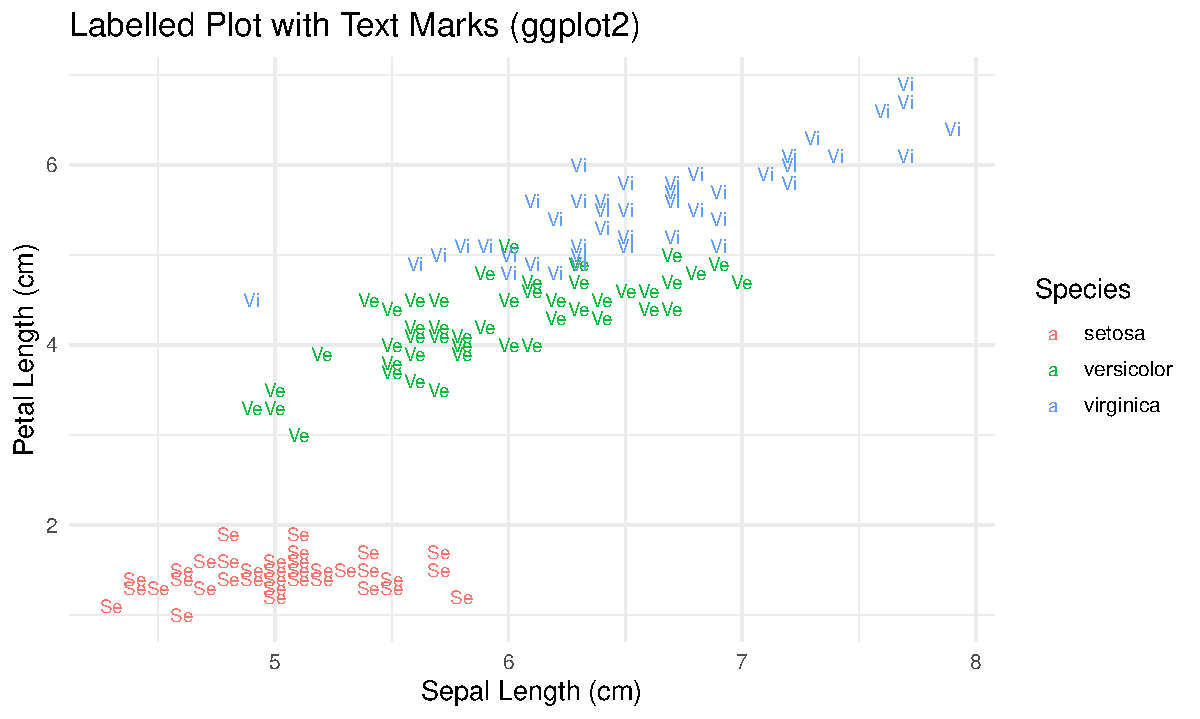
\includegraphics{vistut_files/figure-pdf/unnamed-chunk-11-1.pdf}
\end{center}

\subsubsection{Step 4: discussion (what ggplot is doing for
you)}\label{step-4-discussion-what-ggplot-is-doing-for-you}

\begin{itemize}
\tightlist
\item
  In \textbf{Base R}, you had to remember a special trick:
  \texttt{type\ =\ "n"} to make a blank canvas, then \texttt{text(...)}
  to place labels.
\item
  In \textbf{ggplot2}, you use the same pattern as always:

  \begin{itemize}
  \tightlist
  \item
    \texttt{ggplot(data,\ aes(...))} to declare meaning
  \item
    \texttt{+\ geom\_text()} to choose the mark
  \item
    \texttt{+\ labs()} and \texttt{+\ theme\_*()} for readability
  \end{itemize}
\item
  This consistency is a big reason ggplot is easier for beginners.
\end{itemize}

\begin{tcolorbox}[enhanced jigsaw, opacitybacktitle=0.6, left=2mm, bottomrule=.15mm, coltitle=black, opacityback=0, toptitle=1mm, title=\textcolor{quarto-callout-warning-color}{\faExclamationTriangle}\hspace{0.5em}{Warning}, colbacktitle=quarto-callout-warning-color!10!white, breakable, colback=white, rightrule=.15mm, colframe=quarto-callout-warning-color-frame, bottomtitle=1mm, arc=.35mm, titlerule=0mm, toprule=.15mm, leftrule=.75mm]

\textbf{Principle (avoid ambiguous encodings):} two classes share the
same initial (``v''). If you use text marks, choose labels that are
\textbf{unique} and \textbf{legible} (e.g., ``Se'', ``Ve'', ``Vi''), or
use colour + shape, or facets.

\end{tcolorbox}

\begin{center}\rule{0.5\linewidth}{0.5pt}\end{center}

\subsection{4 --- Small multiples: Base R vs ggplot2
facets}\label{small-multiples-base-r-vs-ggplot2-facets}

\subsubsection{Goal}\label{goal-3}

Create \textbf{three random subsets} of \texttt{iris} and show them
side-by-side to compare patterns.

Key requirement:

\begin{itemize}
\tightlist
\item
  all panels must share the \textbf{same axis limits} so comparisons are
  valid.
\end{itemize}

\subsubsection{Step 1: Base R version (shown
first)}\label{step-1-base-r-version-shown-first-3}

This is a classic situation where ggplot tends to feel easier:
\textbf{small multiples} (many similar plots side-by-side).

In Base R you typically have to:

\begin{itemize}
\tightlist
\item
  set the layout manually (\texttt{par(mfrow\ =\ ...)})
\item
  use a loop to draw each panel
\item
  fix axis limits yourself so the panels are comparable
\end{itemize}

Here is the Base R code:

\begin{Shaded}
\begin{Highlighting}[]
\FunctionTok{set.seed}\NormalTok{(}\DecValTok{123}\NormalTok{)}
\NormalTok{n\_subsets }\OtherTok{\textless{}{-}} \DecValTok{3}
\NormalTok{subset\_size }\OtherTok{\textless{}{-}} \DecValTok{50}

\NormalTok{xlim }\OtherTok{\textless{}{-}} \FunctionTok{range}\NormalTok{(iris}\SpecialCharTok{$}\NormalTok{Sepal.Length)}
\NormalTok{ylim }\OtherTok{\textless{}{-}} \FunctionTok{range}\NormalTok{(iris}\SpecialCharTok{$}\NormalTok{Petal.Length)}

\FunctionTok{par}\NormalTok{(}\AttributeTok{mfrow =} \FunctionTok{c}\NormalTok{(}\DecValTok{1}\NormalTok{, n\_subsets), }\AttributeTok{mar =} \FunctionTok{c}\NormalTok{(}\DecValTok{4}\NormalTok{, }\DecValTok{4}\NormalTok{, }\DecValTok{3}\NormalTok{, }\DecValTok{1}\NormalTok{))}

\ControlFlowTok{for}\NormalTok{ (i }\ControlFlowTok{in} \DecValTok{1}\SpecialCharTok{:}\NormalTok{n\_subsets) \{}
\NormalTok{  sub }\OtherTok{\textless{}{-}}\NormalTok{ iris[}\FunctionTok{sample}\NormalTok{(}\FunctionTok{nrow}\NormalTok{(iris), subset\_size), ]}
  \FunctionTok{plot}\NormalTok{(}
\NormalTok{    sub}\SpecialCharTok{$}\NormalTok{Sepal.Length, sub}\SpecialCharTok{$}\NormalTok{Petal.Length,}
    \AttributeTok{col =} \FunctionTok{as.numeric}\NormalTok{(sub}\SpecialCharTok{$}\NormalTok{Species),}
    \AttributeTok{pch =} \DecValTok{16}\NormalTok{,}
    \AttributeTok{xlim =}\NormalTok{ xlim, }\AttributeTok{ylim =}\NormalTok{ ylim,}
    \AttributeTok{xlab =} \StringTok{"Sepal Length"}\NormalTok{, }\AttributeTok{ylab =} \StringTok{"Petal Length"}\NormalTok{,}
    \AttributeTok{main =} \FunctionTok{paste}\NormalTok{(}\StringTok{"Subset"}\NormalTok{, i)}
\NormalTok{  )}
\NormalTok{\}}
\end{Highlighting}
\end{Shaded}

\begin{center}
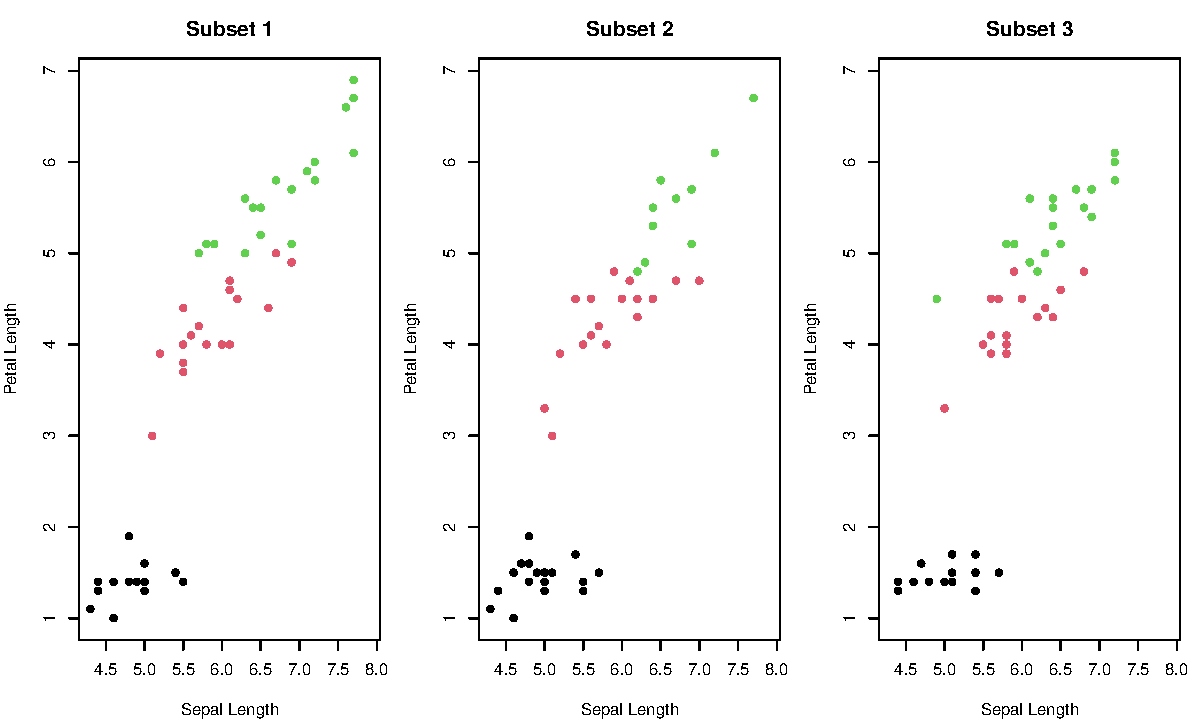
\includegraphics{vistut_files/figure-pdf/unnamed-chunk-12-1.pdf}
\end{center}

\begin{Shaded}
\begin{Highlighting}[]
\FunctionTok{par}\NormalTok{(}\AttributeTok{mfrow =} \FunctionTok{c}\NormalTok{(}\DecValTok{1}\NormalTok{, }\DecValTok{1}\NormalTok{))}
\end{Highlighting}
\end{Shaded}

\subsubsection{Step 2: pause and predict the ggplot2
version}\label{step-2-pause-and-predict-the-ggplot2-version-3}

Now think in ggplot terms:

\begin{itemize}
\tightlist
\item
  ``If I had one table where every row is a point, and I add a column
  called \texttt{Subset}, then I can facet by that column.''
\end{itemize}

So your prediction should be:

\begin{itemize}
\tightlist
\item
  create a column \texttt{Subset}
\item
  draw one scatter plot
\item
  ask ggplot to split into panels with
  \texttt{facet\_wrap(\textasciitilde{}\ Subset)}
\end{itemize}

\subsubsection{Step 3: ggplot2 version
(solution)}\label{step-3-ggplot2-version-solution-3}

\begin{Shaded}
\begin{Highlighting}[]
\FunctionTok{set.seed}\NormalTok{(}\DecValTok{123}\NormalTok{)}
\NormalTok{n\_subsets }\OtherTok{\textless{}{-}} \DecValTok{3}
\NormalTok{subset\_size }\OtherTok{\textless{}{-}} \DecValTok{50}

\NormalTok{subset\_list }\OtherTok{\textless{}{-}} \FunctionTok{lapply}\NormalTok{(}\DecValTok{1}\SpecialCharTok{:}\NormalTok{n\_subsets, }\ControlFlowTok{function}\NormalTok{(i) \{}
\NormalTok{  sub }\OtherTok{\textless{}{-}}\NormalTok{ iris[}\FunctionTok{sample}\NormalTok{(}\FunctionTok{nrow}\NormalTok{(iris), subset\_size), ]}
\NormalTok{  sub}\SpecialCharTok{$}\NormalTok{Subset }\OtherTok{\textless{}{-}} \FunctionTok{paste}\NormalTok{(}\StringTok{"Subset"}\NormalTok{, i)}
\NormalTok{  sub}
\NormalTok{\})}
\NormalTok{iris\_subs }\OtherTok{\textless{}{-}} \FunctionTok{do.call}\NormalTok{(rbind, subset\_list)}

\FunctionTok{ggplot}\NormalTok{(iris\_subs, }\FunctionTok{aes}\NormalTok{(Sepal.Length, Petal.Length, }\AttributeTok{colour =}\NormalTok{ Species)) }\SpecialCharTok{+}
  \FunctionTok{geom\_point}\NormalTok{(}\AttributeTok{size =} \DecValTok{2}\NormalTok{) }\SpecialCharTok{+}
  \FunctionTok{scale\_color\_manual}\NormalTok{(}\AttributeTok{values =} \FunctionTok{c}\NormalTok{(}\StringTok{"darkgreen"}\NormalTok{, }\StringTok{"steelblue"}\NormalTok{, }\StringTok{"darkorange"}\NormalTok{)) }\SpecialCharTok{+}
  \FunctionTok{coord\_cartesian}\NormalTok{(}
    \AttributeTok{xlim =} \FunctionTok{range}\NormalTok{(iris}\SpecialCharTok{$}\NormalTok{Sepal.Length),}
    \AttributeTok{ylim =} \FunctionTok{range}\NormalTok{(iris}\SpecialCharTok{$}\NormalTok{Petal.Length)}
\NormalTok{  ) }\SpecialCharTok{+}
  \FunctionTok{facet\_wrap}\NormalTok{(}\SpecialCharTok{\textasciitilde{}}\NormalTok{ Subset) }\SpecialCharTok{+}
  \FunctionTok{labs}\NormalTok{(}
    \AttributeTok{x =} \StringTok{"Sepal Length (cm)"}\NormalTok{,}
    \AttributeTok{y =} \StringTok{"Petal Length (cm)"}\NormalTok{,}
    \AttributeTok{colour =} \StringTok{"Species"}\NormalTok{,}
    \AttributeTok{title =} \StringTok{"Random Subsets of the Iris Dataset"}
\NormalTok{  ) }\SpecialCharTok{+}
  \FunctionTok{theme\_minimal}\NormalTok{(}\AttributeTok{base\_size =} \DecValTok{13}\NormalTok{) }\SpecialCharTok{+}
  \FunctionTok{theme}\NormalTok{(}\AttributeTok{legend.position =} \StringTok{"bottom"}\NormalTok{)}
\end{Highlighting}
\end{Shaded}

\begin{center}
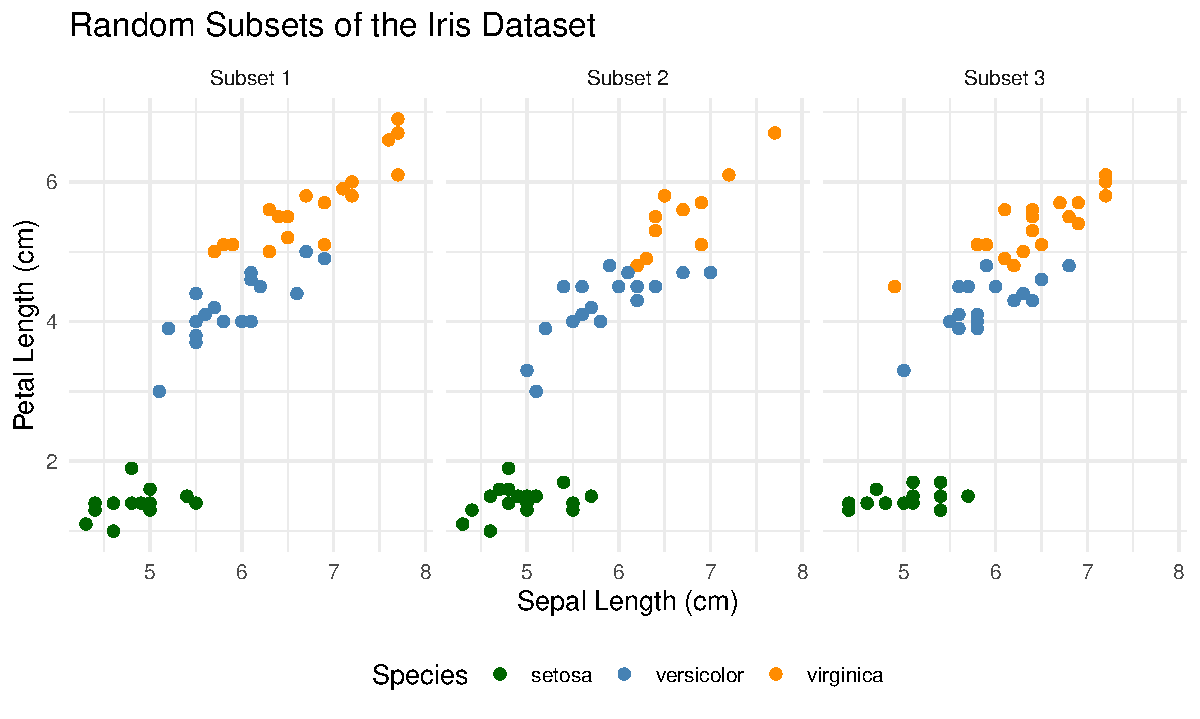
\includegraphics{vistut_files/figure-pdf/unnamed-chunk-13-1.pdf}
\end{center}

\subsubsection{Step 4: discussion (why ggplot2 is ``scalable''
here)}\label{step-4-discussion-why-ggplot2-is-scalable-here}

\begin{itemize}
\tightlist
\item
  In \textbf{Base R}, making 10 panels means more layout thinking, more
  looping, and more manual control.
\item
  In \textbf{ggplot2}, the plot code stays almost the same. You mostly
  change the \textbf{data} (more rows / more subsets), and ggplot keeps
  the layout consistent.
\item
  This is one of the main advantages of the Grammar of Graphics
  approach: once the mapping is declared, ``many panels'' becomes a data
  problem, not a drawing problem.
\end{itemize}

\begin{tcolorbox}[enhanced jigsaw, opacitybacktitle=0.6, left=2mm, bottomrule=.15mm, coltitle=black, opacityback=0, toptitle=1mm, title=\textcolor{quarto-callout-note-color}{\faInfo}\hspace{0.5em}{Note}, colbacktitle=quarto-callout-note-color!10!white, breakable, colback=white, rightrule=.15mm, colframe=quarto-callout-note-color-frame, bottomtitle=1mm, arc=.35mm, titlerule=0mm, toprule=.15mm, leftrule=.75mm]

\textbf{Principles used}

\begin{itemize}
\tightlist
\item
  \textbf{Small multiples}: comparisons become easier when panels share
  scales and design.
\item
  \textbf{Consistency beats decoration}: repeatable structure reduces
  cognitive load.
\item
  \textbf{Grammar of Graphics}: once the mapping is declared, faceting
  is a data operation rather than a manual layout job.
\end{itemize}

\end{tcolorbox}

\begin{center}\rule{0.5\linewidth}{0.5pt}\end{center}

\subsection{5 --- Scatter + smoother + scale
thinking}\label{scatter-smoother-scale-thinking}

\subsubsection{Goal}\label{goal-4}

Add a group-wise smoother to \texttt{Sepal.Length} vs
\texttt{Petal.Length}:

\begin{itemize}
\tightlist
\item
  Base R: \texttt{lowess()} per species
\item
  ggplot2: \texttt{geom\_smooth(method\ =\ "loess")}
\end{itemize}

Also practice \textbf{scale discipline}:

\begin{itemize}
\tightlist
\item
  choose breaks intentionally
\item
  label them clearly
\end{itemize}

\subsubsection{Step 1: Base R version (shown
first)}\label{step-1-base-r-version-shown-first-4}

In Base R, adding a ``trend line'' per group usually means:

\begin{itemize}
\tightlist
\item
  draw the scatter plot
\item
  split the data by group (Species)
\item
  for each group, compute a smoother (here we use \texttt{lowess(...)})
\item
  draw that smoother line with \texttt{lines(...)}
\end{itemize}

Here is the Base R code:

\begin{Shaded}
\begin{Highlighting}[]
\FunctionTok{plot}\NormalTok{(}
\NormalTok{  iris}\SpecialCharTok{$}\NormalTok{Sepal.Length, iris}\SpecialCharTok{$}\NormalTok{Petal.Length,}
  \AttributeTok{col =} \FunctionTok{as.numeric}\NormalTok{(iris}\SpecialCharTok{$}\NormalTok{Species),}
  \AttributeTok{pch =} \DecValTok{16}\NormalTok{,}
  \AttributeTok{xlab =} \StringTok{"Sepal Length"}\NormalTok{,}
  \AttributeTok{ylab =} \StringTok{"Petal Length (cm)"}\NormalTok{,}
  \AttributeTok{main =} \StringTok{"Sepal vs Petal Length with Mean Smoother"}
\NormalTok{)}

\ControlFlowTok{for}\NormalTok{ (i }\ControlFlowTok{in} \DecValTok{1}\SpecialCharTok{:}\DecValTok{3}\NormalTok{) \{}
\NormalTok{  sub }\OtherTok{\textless{}{-}}\NormalTok{ iris[iris}\SpecialCharTok{$}\NormalTok{Species }\SpecialCharTok{==} \FunctionTok{levels}\NormalTok{(iris}\SpecialCharTok{$}\NormalTok{Species)[i], ]}
  \FunctionTok{lines}\NormalTok{(}\FunctionTok{lowess}\NormalTok{(sub}\SpecialCharTok{$}\NormalTok{Sepal.Length, sub}\SpecialCharTok{$}\NormalTok{Petal.Length), }\AttributeTok{col =}\NormalTok{ i, }\AttributeTok{lwd =} \DecValTok{2}\NormalTok{)}
\NormalTok{\}}

\FunctionTok{legend}\NormalTok{(}
  \StringTok{"topleft"}\NormalTok{,}
  \AttributeTok{legend =} \FunctionTok{levels}\NormalTok{(iris}\SpecialCharTok{$}\NormalTok{Species),}
  \AttributeTok{col =} \DecValTok{1}\SpecialCharTok{:}\DecValTok{3}\NormalTok{, }\AttributeTok{pch =} \DecValTok{16}\NormalTok{, }\AttributeTok{lwd =} \DecValTok{2}\NormalTok{,}
  \AttributeTok{title =} \StringTok{"Iris Species"}
\NormalTok{)}
\end{Highlighting}
\end{Shaded}

\begin{center}
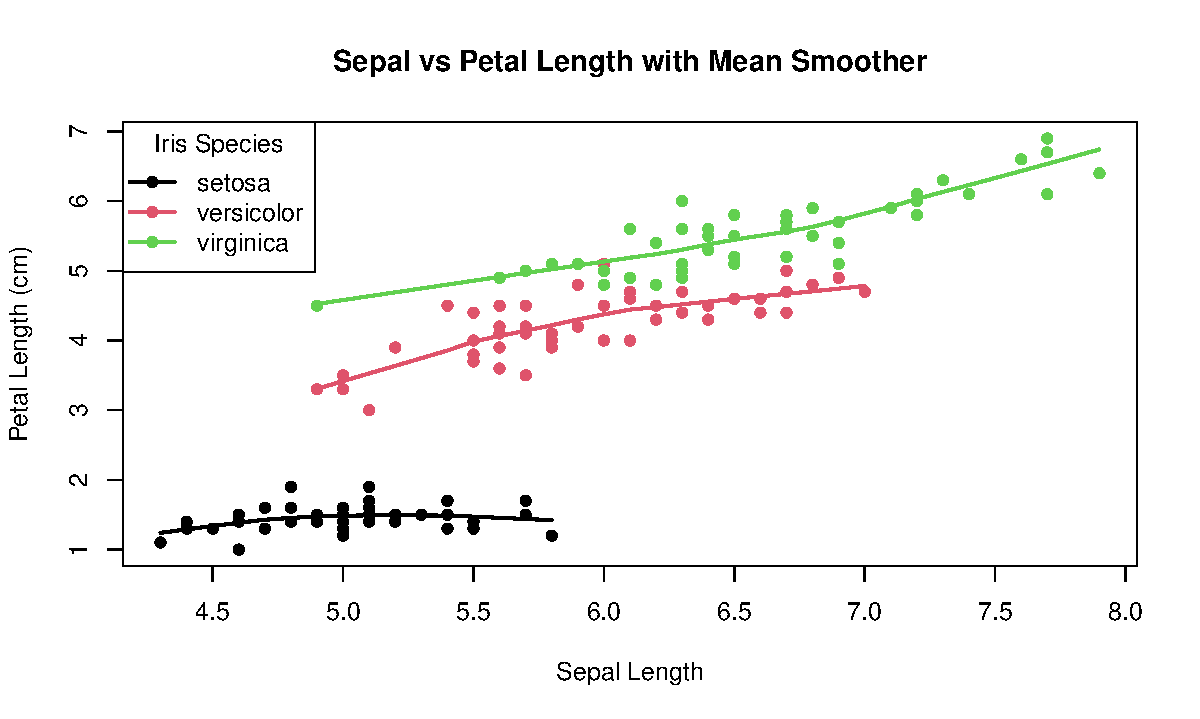
\includegraphics{vistut_files/figure-pdf/unnamed-chunk-14-1.pdf}
\end{center}

\subsubsection{Step 2: pause and predict the ggplot2
version}\label{step-2-pause-and-predict-the-ggplot2-version-4}

In ggplot2, the ``translation'' is usually:

\begin{itemize}
\tightlist
\item
  points → \texttt{geom\_point()}
\item
  smoother → \texttt{geom\_smooth()}
\item
  grouping by Species happens automatically because colour is mapped to
  Species
\end{itemize}

So before you look, predict what the ggplot sentence will look like:

\begin{itemize}
\tightlist
\item
  start: \texttt{ggplot(iris,\ aes(...))}
\item
  then: \texttt{+\ geom\_point(...)}
\item
  then: \texttt{+\ geom\_smooth(...)}
\item
  then: labels and theme
\end{itemize}

\subsubsection{Step 3: ggplot2 version
(solution)}\label{step-3-ggplot2-version-solution-4}

\begin{Shaded}
\begin{Highlighting}[]
\FunctionTok{ggplot}\NormalTok{(iris, }\FunctionTok{aes}\NormalTok{(}\AttributeTok{x =}\NormalTok{ Sepal.Length, }\AttributeTok{y =}\NormalTok{ Petal.Length, }\AttributeTok{colour =}\NormalTok{ Species)) }\SpecialCharTok{+}
  \FunctionTok{geom\_point}\NormalTok{(}\AttributeTok{size =} \DecValTok{2}\NormalTok{, }\AttributeTok{alpha =} \FloatTok{0.7}\NormalTok{) }\SpecialCharTok{+}
  \FunctionTok{geom\_smooth}\NormalTok{(}\AttributeTok{se =} \ConstantTok{FALSE}\NormalTok{, }\AttributeTok{method =} \StringTok{"loess"}\NormalTok{, }\AttributeTok{linewidth =} \FloatTok{1.2}\NormalTok{) }\SpecialCharTok{+}
  \FunctionTok{scale\_color\_manual}\NormalTok{(}
    \AttributeTok{values =} \FunctionTok{c}\NormalTok{(}\StringTok{"darkgreen"}\NormalTok{, }\StringTok{"steelblue"}\NormalTok{, }\StringTok{"darkorange"}\NormalTok{),}
    \AttributeTok{name =} \StringTok{"Iris Species"}
\NormalTok{  ) }\SpecialCharTok{+}
  \FunctionTok{labs}\NormalTok{(}
    \AttributeTok{x =} \StringTok{"Sepal Length (cm)"}\NormalTok{,}
    \AttributeTok{y =} \StringTok{"Petal Length (cm)"}\NormalTok{,}
    \AttributeTok{title =} \StringTok{"Sepal vs Petal Length with Mean Smoother"}
\NormalTok{  ) }\SpecialCharTok{+}
  \FunctionTok{theme\_minimal}\NormalTok{(}\AttributeTok{base\_size =} \DecValTok{13}\NormalTok{)}
\end{Highlighting}
\end{Shaded}

\begin{center}
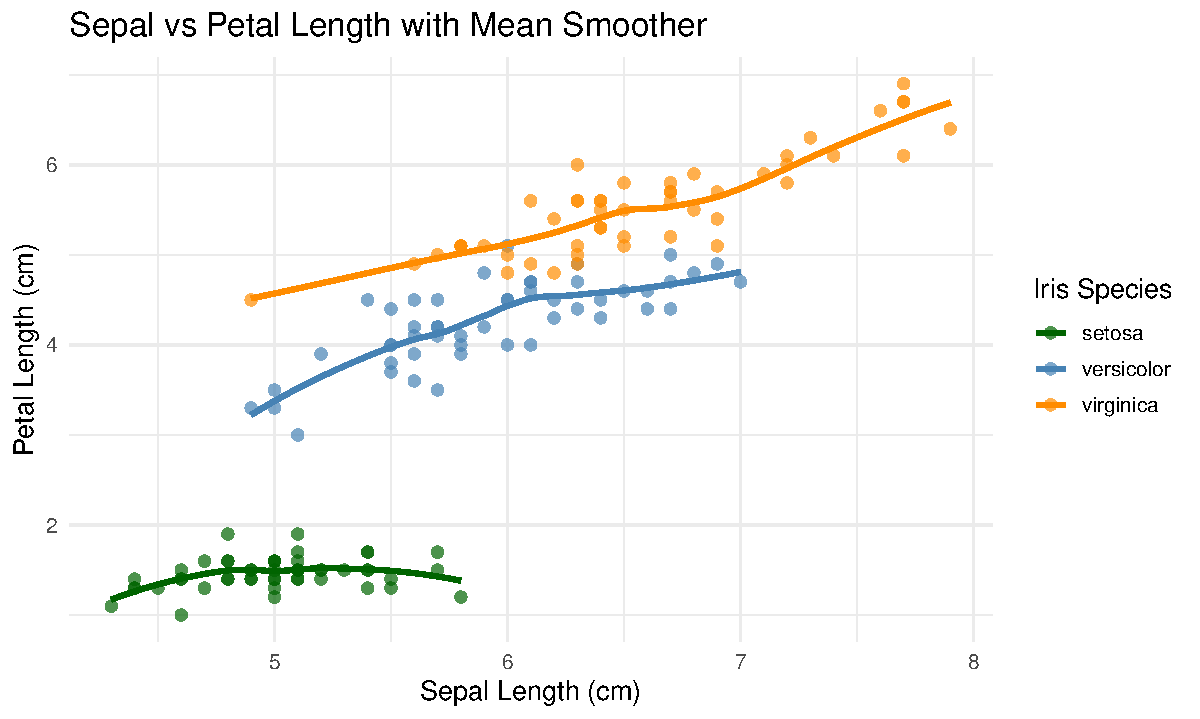
\includegraphics{vistut_files/figure-pdf/unnamed-chunk-15-1.pdf}
\end{center}

\subsubsection{Step 4: discussion (what is simpler in
ggplot2)}\label{step-4-discussion-what-is-simpler-in-ggplot2}

\begin{itemize}
\tightlist
\item
  In \textbf{Base R}, you manually looped over species and manually drew
  each smoother line.
\item
  In \textbf{ggplot2}, you told ggplot ``colour means Species'', and
  ggplot uses that grouping to draw separate smoothers automatically.
\item
  This is the same ``consistency advantage'' again: you add layers, and
  ggplot handles grouping + legends in a predictable way.
\end{itemize}

\begin{tcolorbox}[enhanced jigsaw, opacitybacktitle=0.6, left=2mm, bottomrule=.15mm, coltitle=black, opacityback=0, toptitle=1mm, title=\textcolor{quarto-callout-warning-color}{\faExclamationTriangle}\hspace{0.5em}{Warning}, colbacktitle=quarto-callout-warning-color!10!white, breakable, colback=white, rightrule=.15mm, colframe=quarto-callout-warning-color-frame, bottomtitle=1mm, arc=.35mm, titlerule=0mm, toprule=.15mm, leftrule=.75mm]

\textbf{Principle (don't let smoothers over-claim):} a smoother is not
``truth''; it's a modelling choice. Always ask:

\begin{itemize}
\tightlist
\item
  Is the smoother appropriate for the data density and noise?
\item
  Would a linear model or summary by bins be clearer?
\item
  Should you show uncertainty (SE/CI ribbon) or keep it simple?
\end{itemize}

\end{tcolorbox}

\begin{center}\rule{0.5\linewidth}{0.5pt}\end{center}

\subsection{Mini-section --- Visualisation principles
checklist}\label{mini-section-visualisation-principles-checklist}

Before you submit a figure, check:

\begin{itemize}
\tightlist
\item
  \textbf{Integrity}: are scales honest? any distortion? any unnecessary
  ink?
\item
  \textbf{Perception}:

  \begin{itemize}
  \tightlist
  \item
    proximity: are related items grouped?
  \item
    similarity: are colours/shapes consistent?
  \item
    figure--ground: is the data visually dominant?
  \end{itemize}
\item
  \textbf{Structure (Grammar of Graphics)}:

  \begin{itemize}
  \tightlist
  \item
    are mappings (\texttt{aes}) explicit and consistent across plots?
  \item
    are scales and guides clearly labelled?
  \end{itemize}
\item
  \textbf{Accessibility}:

  \begin{itemize}
  \tightlist
  \item
    can it be read in grayscale?
  \item
    is colour the \emph{only} encoding?
  \item
    is text large enough for projection/print?
  \end{itemize}
\end{itemize}

\begin{center}\rule{0.5\linewidth}{0.5pt}\end{center}

\subsection{Optional extensions}\label{optional-extensions}

\subsubsection{Extension 1 --- Make labels
unambiguous}\label{extension-1-make-labels-unambiguous}

Replace initials with unique labels: ``Se'', ``Ve'', ``Vi''.

\subsubsection{Extension 2 --- Use facets to replace
colour}\label{extension-2-use-facets-to-replace-colour}

Create a \texttt{facet\_wrap(\textasciitilde{}\ Species)} plot and move
legend off (or drop colour entirely).

\subsubsection{Extension 3 --- Write a ``caption that completes the
figure''}\label{extension-3-write-a-caption-that-completes-the-figure}

Write 3--4 sentences:

\begin{itemize}
\tightlist
\item
  what is shown (variables + units)
\item
  what colour encodes
\item
  what the smoother means (if present)
\item
  what the key takeaway is (one sentence)
\end{itemize}

\begin{center}\rule{0.5\linewidth}{0.5pt}\end{center}

\subsection{Wrap-up}\label{wrap-up}

You now have a repeatable workflow:

\begin{itemize}
\tightlist
\item
  start with the \textbf{question}
\item
  choose encodings that support perception (Gestalt)
\item
  keep figures honest and minimal (Tufte)
\item
  build plots as structured statements (Grammar of Graphics)
\end{itemize}




\end{document}
